\subsection{Filtro de Color (fcolor)}
	\subsubsection{Idea}
		La idea de este filtro es dado un video y un color determinado por la tupla de valores $(rc,gc,bc)$ y un valor de tolerancia $threshold$ poder procesar el video de forma que los colores cuya distancia eucl\'idea a $(rc,gc,bc)$ sea mayor a $threshold$ deb\'ian ser cambiados a escala de grises. Aquellos valores que no cumpl\'ian esa condici\'on no eran modificados.
		
	\subsubsection{Implementaci\'on en C}
	
	A continuaci\'on se expresa en pseudoc\'odigo la implementaci\'on en C.
	
	\begin{algorithmic}[1]
		\State int $pixelActual$ $\gets$ 0;
		\State int $cantPixeles$ $\gets$ $width$ $\times$ $height$;
		\While{$pixelActual$ < $cantPixeles$}
			\State unsigned char $rojo$ $\gets$ $pixelActual$.r;
			\State unsigned char $verde$ $\gets$ $pixelActual$.g;
			\State unsigned char $azul$ $\gets$ $pixelActual$.b;
			\If{distancia(($rojo$,$verde$,$azul$),($rc$,$gc$,$bc$)) > $threshold$}
				\State unsigned char $gris$ $\gets$ (($rojo$+$verde$+$azul$)/3);
				\State $pixelActual$.r $\gets$ $gris$;
				\State $pixelActual$.g $\gets$ $gris$;
				\State $pixelActual$.b $\gets$ $gris$;
			\EndIf
			\State $pixelActual$++;
		\EndWhile
	\end{algorithmic}

	B\'asicamente el c\'odigo en $C$ realiza ese procedimiento. A la hora de calcular distancia tiene que hacer ciertas salvedades:
	
	\begin{itemize}
		\item Pasar unsigned char a int.
		\item Restarles a cada valor su correspondiente valor de ($rc$,$gc$,$bc$).
		\item Elevar cada valor al cuadrado y realizar la suma.
		\item A la hora de calcular la ra\'iz cuadrada se utiliza una conversi\'on a double.
		\item Luego ese valor es redondeado hacia arriba a int.\footnotemark[1]
	\end{itemize}
	
	(1) El redondeo se realiza para arriba para preservar que si el valor en double era mayor al threshold entonces el valor en entero lo va a seguir siendo.

	
	\subsubsection{Implementaci\'on en ASM}
	
	La implementaci\'on en $ASM$ conserva el mismo espirit\'u de la implementaci\'on en $C$ pero en vez de procesar de a un p\'ixel por vez lo hace de a 4 p\'ixeles aprovechando los registros es instrucciones que brinda $SSE$. Otra diferencia principal es que el c\'alculo de grises se realiza para todos los p\'ixeles independientemente que cumplan o no la condici\'on de filtrado; esto realiza las cuentas m\'as directas y s\'olo es necesario obtener con una m\'ascara el \'indice de los p\'ixeles a cambiar. Se proceder\'a a explicar una iteraci\'on del c\'odigo con im\'agenes. Intercalaremos comentarios acerca de la conversi\'on de datos.
	
	Lo que est\'a sombreado de gris es aquello que no importa su contenido porque es descartado o ignorado a la hora de hacer cuentas. 
	
	\begin{figure}[H]
		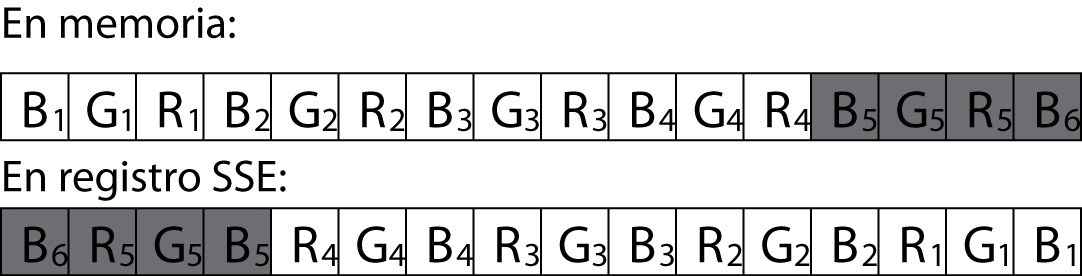
\includegraphics[scale=0.9]{imgs/fcolor_asm1.png}
		\caption{Al comienzo, tenemos en memoria los p\'ixeles del frame a filtrar. Al cargar esos datos en un registro $SSE$ se observa que el orden de los elementos se invierte.} 
	\end{figure}
	
	\begin{figure}[H]
		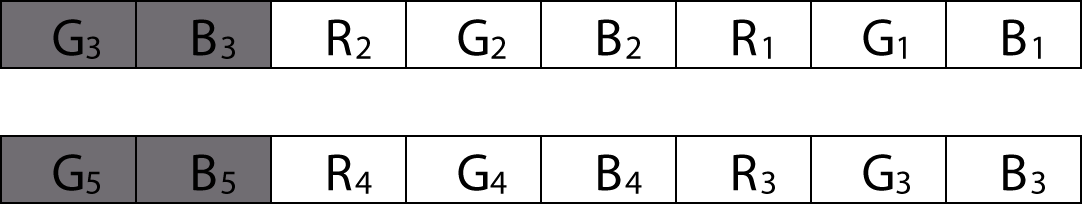
\includegraphics[scale=0.9]{imgs/fcolor_asm2.png}
		\caption{Desempaquetamos en 2 registros distintos con las instrucciones punpckXbw de modo que los valores que eran unsigned char de 1 byte est\'en ahora almacenados en 2 bytes, permiti\'endonos hacer operaciones con ellos sin riesgo de overflow.}
	\end{figure}
	
	Vamos a continuar mostrando el procedimiento con uno s\'olo de esos registros,al otro le realizamos el mismo proceso y en un momento se juntan los resultados.
	
	\begin{figure}[H]
		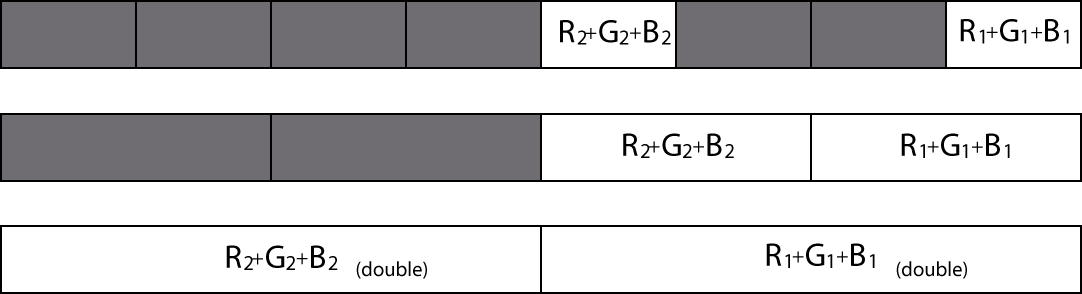
\includegraphics[scale=0.9]{imgs/fcolor_asm3.png}
		\caption{Luego con shifteos hacia derecha ($PSRLDQ$) y sumas de valores empaquetados obtenemos para cada uno de esos registros la suma de los valores de cada canal para esos 4 p\'ixeles. Aumentamos la precisi\'on porque para convertir a punto flotante necesito tener dwords. Y convertimos a punto flotante para hacer la divisi\'on.}
	\end{figure}
	
	\begin{figure}[H]
		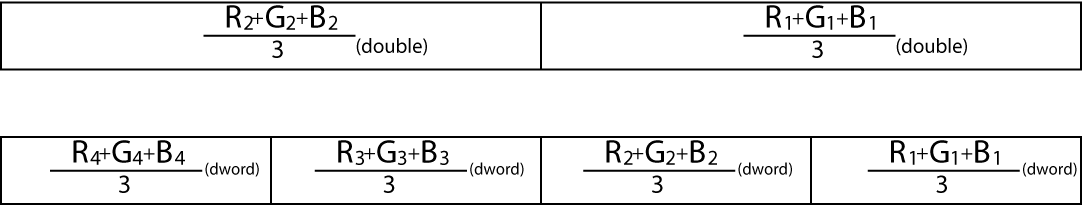
\includegraphics[scale=0.9]{imgs/fcolor_asm4.png}
		\caption{Luego de realizar la divisi\'on por 3 volvemos a convertir los valores a dwords, redondeando normalmente. Y nuevamente seguimos convirtiendo a hasta que los valores quedan como bytes, como estaban originalmente. Es notable observar que el valor hallado con la divisi\'on entra bien en un byte, de modo que no hay que hacer saturaci\'on para convertir a tipos m\'as peque\~nos.}
	\end{figure}
	
	\begin{figure}[H]
		
\includegraphics[scale=0.9]{imgs/fcolor_asm5.png}
		\caption{Para finalizar, utilizando la instrucci\'on $PSHUFB$ hacemos un broadcast(repetici\'on de datos por todo el registro) de los valores hallados de modo que a cada p\'ixel le corresponda en los tres canales el valor de gris calculado.}
	\end{figure}
	
	\begin{figure}[H]
		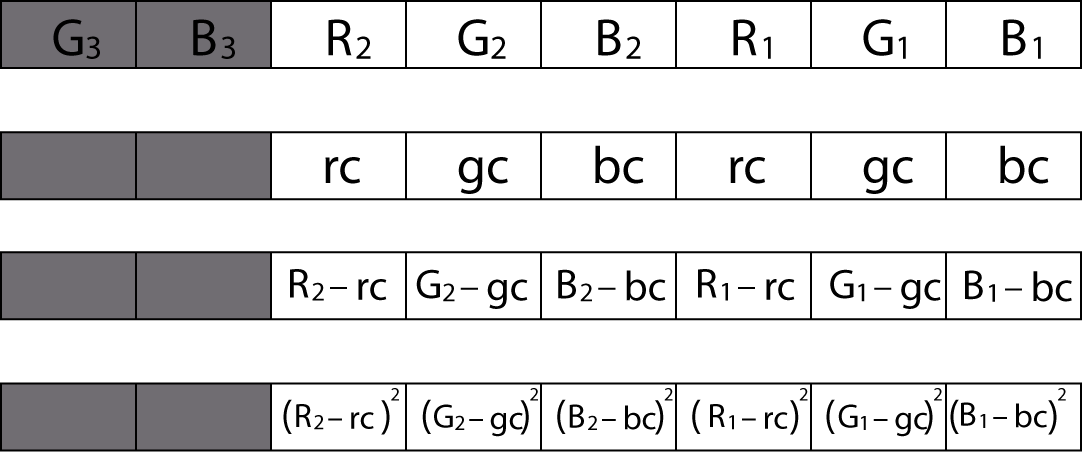
\includegraphics[scale=0.9]{imgs/fcolor_asm6.png}
		\caption{Ahora procedemos a realizar el c\'alculo de distancias para decidir que valores debemos filtrar. Para ello tenemos cargado en memoria una posici\'on de memoria con los valores rc, gc y bc para poder levantarlos con los registros de $SSE$.Hacemos la resta con esos valores para luego elevarlos al cuadrado. }
	\end{figure}
	
	N\'otese que por ahora los valores, que originalmente proven\'ian de un unsigned char est\'an en words, y elevarlos al cuadrado todav\'ia est\'a dentro de los l\'imites de los words. Sin embargo, ahora debemos realizar la suma de los valores elevados al cuadrado, y ah\'i no lo podemos hacer en words, as\'i que nuevamente convertimos a dwords.
	
	\begin{figure}[H]
		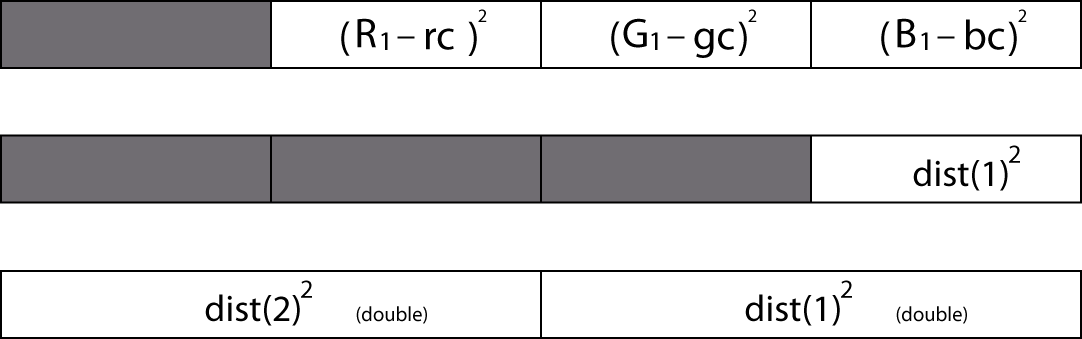
\includegraphics[scale=0.9]{imgs/fcolor_asm7.png}
		\caption{Con dwords puedo realizar las sumas sin problemas. Despu\'es vamos a necesitar calcular la ra\'iz cuadrada de los valores hallados, y es por esta raz\'on que convertimos los valores a doubles empaquetados.}
	\end{figure}
	
	\begin{figure}[H]
		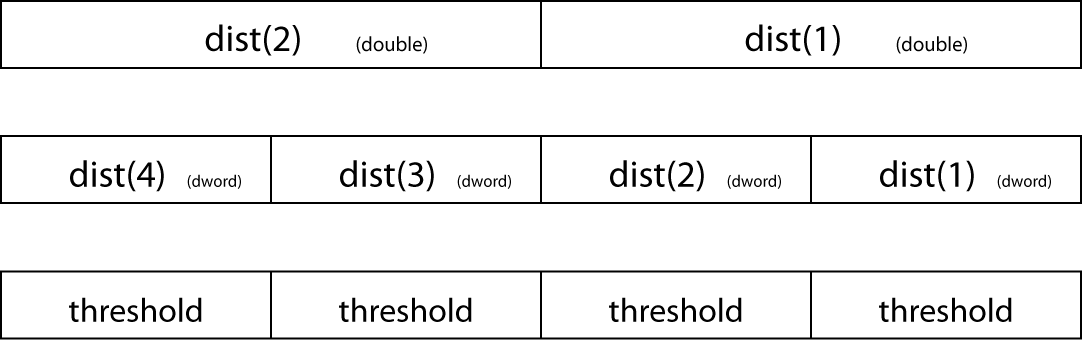
\includegraphics[scale=0.9]{imgs/fcolor_asm8.png}
		\caption{Calculamos la ra\'iz cuadrada de esos valores. Luego convertimos con redondeo hacia arriba a dwords fusionando las distancias de cada uno de los 4 p\'ixeles en un mismo registro. Ah\'i es donde realizamos la comparaci\'on para ver cu\'al de esas distancias es mayor a $threshold$(antes cargamos en un registro de $SSE$ estos valores para poder realizar la comparaci\'on).}
	\end{figure}
	
	Utilizando la m\'ascara como resultado y los valores de gris ya calculados realiz\'o una uni\'on de valores de modo que al final en un registro tenga juntos los valores en escala de grises junto a los valores no modificados, seg\'un se haya cumplido o no la condici\'on.
	
	
	Para finalizar se escribe dicho registro en la direcci\'on de memoria correspondiente al frame modificado, se avanza los punteros del frame original y del frame destino en 12 bytes(por los 4 p\'ixeles procesados en la iteraci\'on) y se vuelve a iterar si es que no termin\'o.

	
	\subsubsection{Diferencias estructurales}
	
		Al comparar el c\'odigo desensamblado de color$\_$filter$\_$c con el código desensamblado de color$\_$filter$\_$asm la principal diferencia que se encuentra es que el código generado por el ensamblador para color$\_$filter$\_$asm es muy similar al código fuente, mientras que no sucede de la misma manera con el código fuente en C.

		El código en C procesa cada cuadro del video de a un pixel por vez, mientras que el código en lenguaje ensamblador procesa de a 4. Además, el código de lenaguaje ensamblador utiliza mucho más los registros e instrucciones relacionadas a SSE, mientras que el código desensamblado de C los utiliza solamente para cálculos de punto flotante.

		En la implementación en C se utiliza bastante el recurso de variables locales y como se puede observar en el código desensamblado dichas variables locales se almacenan en el stack, y por cada operación que las involucrase se tiene que acceder a memoria; esto en lenguaje ensamblador no sucede, ya que se utilizan los registros de propósito general y los registros SSE, reduciendo considerablemente la cantidad de accesos a memoria y por ende mejorando la performance. Dicho esto, se puede observar que el código generado por la implementación en C podría optimizarse utilizando más registros de propósito general.
	
	\subsubsection{Optimizaci\'on de C}
	
	\paragraph{Opciones de compilaci\'on}
	
		Compilar el código en C con la opción -O1 significa que va a tratar de optimizar el código de manera que se ejecute más rápido; para lograr esto el tiempo de compilación va a aumentar ya que tiene que hacer más trabajo. En nuestro caso, el código es relativamente simple, por lo tanto el tiempo de compilación no tuvo grandes diferencias con la versión sin optimizaciones.

		Una de las principales diferencias entre el código no optimizado y el código compilado con -O1 es que se utiilizan más los registros de propósito general en vez de utilizar memoria para almacenar las variables locales. Como era de esperarse, eso trajo consigo una mayor performance a la hora de aplicar el filtro.

		También el código generado no respeta el orden de las instrucciones en el código C, por ejemplo:
		
\vspace{1 cm}

(C\'odigo sin opciones de optimizaci\'on)
\begin{verbatim}
        red = red - rc_i;
    5c: 8b 45 f0             	mov    -0x10(%rbp),%eax
    5f: 29 45 e4             	sub    %eax,-0x1c(%rbp)
        red = red*red;
    62: 8b 45 e4             	mov    -0x1c(%rbp),%eax
    65: 0f af 45 e4          	imul   -0x1c(%rbp),%eax
    69: 89 45 e4             	mov    %eax,-0x1c(%rbp)
\end{verbatim}

\vspace{1 cm}

(C\'odigo con -O1)
\begin{verbatim}

        red = red - rc_i;
    15: 44 89 ce             	mov    %r9d,%esi
    18: 29 fe                	sub    %edi,%esi
  
    ...Más operaciones de por medio...
  
        red = red*red;
    27: 0f af f6             	imul   %esi,%esi
	
\end{verbatim}
  
  
	Sin embargo, el código optimizado aún no aprovecha todos los registros SSE a su disposición; sólo los utliza cuando tiene que calcular raíces cuadradas o realizar divisiones.

	Se observa también que la performance del filtro en C optimizado con -O1 trabaja casi tan rápido como el de assembler, esto se confirmará cuando se hagan los análisis de tiempo.

	El compilador ofrece otras opciones de optimización como:
	
	\begin{itemize}

	\item -O2: El compilador optimiza aún más y busca conseguir tiempos de compilación y ejecución rápidos. Inlcuye todas las optimizaciones incluídas en -O1. El código puede volverse inestable si utiliza etiquetas "goto".
	
	\item -O3: Incluye las optimizaciones de -O2, y agrega más.
	
	\item -Ofast: Compila dejando de lado estándares de código(IEEE, ISO), pudiendo generar comportamientos inesperados si el código hacía uso de dichos estándares.

	\end{itemize}
	
	\paragraph{Loop unrolling}
	
	La técnica de desenrollado de ciclos ("loop unrolling") es un método para optimizar la ejecución de código, logrando un tiempo más corto. Sin embargo, esta optimización no viene sin costos: aumenta el tamaño de código fuente y de código ejecutable y hay situaciones en las cuales esto no es deseable.

	Para ello, la técnica de "loop unrolling" se encarga de reducir la cantidad de iteraciones de los ciclos y asimismo reducir la cantidad de evaluaciones y saltos condicionales durante la ejecución del programa. Esto se puede lograr reemplazando el contenido de los ciclos de modo que en una iteraci\'on del nuevo c\'odigo haya varias iteraciones del c\'odigo original.

	Considere el siguiente pseudocódigo hecho en C:

\begin{verbatim}
	for(i = 0; i < 100,++i){
	    hacerAccion(i)
	}
\end{verbatim}

Se puede observar que el código hace 100 iteraciones de hacerAcción, teniendo que aumentar el contador para luego evaluar si se cumplió la condición de salida.

Si se aplica la técnica de "loop unrolling", el código queda de la siguiente forma:

\begin{verbatim}
    for(i = 0; i < 100,i+=5){
        hacerAccion(i)
        hacerAccion(i+1)
        hacerAccion(i+2)
        hacerAccion(i+3)
        hacerAccion(i+4)
    }
\end{verbatim}

El código resultante hace 20 iteraciones en vez de 100, y la condición de salida es evaluada 20 veces.

Sin embargo está técnica no puede ser aplicada siempre; hay casos donde la condición de salida involucra otras variables.

En nuestro caso se propone reducir cada ciclo original que procesaba de a 12 píxeles con uno que procesa de a 48 píxeles. Con esto la cantidad total de iteraciones es un 25$\%$ de la cantidad de iteraciones original.
	
	\subsubsection{An\'alisis temporal}
	
	